\documentclass[conference]{IEEEtran}
\usepackage{amsmath}
\usepackage{graphicx}
\usepackage{url}
\usepackage[hidelinks]{hyperref}

\begin{document}

\title{Land Risk Intelligence: An AI-Powered Geospatial Risk Assessment Platform}

\author{ \IEEEauthorblockN{Shardendu Mishra} \IEEEauthorblockA{ 23BCS122 \\ 23bcs122@iiitdwd.ac.in } \and \IEEEauthorblockN{Anas Khan} \IEEEauthorblockA{ 23BCS083 \\ 23bcs083@iiitdwd.ac.in } \and \IEEEauthorblockN{Simone John Rodriguez} \IEEEauthorblockA{ 23BCS111 \\ 23bcs111@iiitdwd.ac.in } \and \IEEEauthorblockN{Niti Priya} \IEEEauthorblockA{ 23BCS087 \\ 23bcs087@iiitdwd.ac.in } }

\maketitle

\begin{abstract}
Land Risk Intelligence is a production-oriented geospatial risk assessment system built with a Go backend, Python ML microservice, and React-Leaflet frontend. The pipeline combines KGIS data pull, geometry preprocessing, satellite feature extraction, model inference, and rule-based validation to generate explainable risk reports with traceable evidence. The implementation is containerized with Docker Compose and backed by PostgreSQL and Redis for persistence and caching. This report presents a repository-grounded analysis of architecture, data flow, technology rationale, deployment model, performance behavior, and frontend experience improvements. It also maps implementation outcomes directly to five evaluation criteria: data pulling and preprocessing, technique and response handling, accuracy and validation, report quality, and frontend design experience.
\end{abstract}

\begin{IEEEkeywords}
geospatial analytics, machine learning systems, microservices, risk assessment, explainable AI
\end{IEEEkeywords}

\section{Introduction}
Land eligibility and compliance assessment requires integrating heterogeneous geospatial sources, converting unstable raw payloads into model-ready features, and producing low-latency results with clear evidence trails. In practical deployments, upstream APIs can vary in latency and schema shape, while user-facing workflows demand immediate clarity about system progress and final confidence.

Land Risk Intelligence addresses this through a layered architecture: synchronous API endpoints for user requests, resilient backend orchestration for data pulling and preprocessing, a dedicated ML service for satellite features and prediction, and an interactive frontend for map-based input and diagnostic visibility. The design goal is not only predictive output, but auditable and explainable decision support under variable external conditions.

\section{System Architecture}
\subsection{Architecture Overview}
The end-to-end flow is: frontend $\rightarrow$ backend API $\rightarrow$ KGIS/ML dependencies $\rightarrow$ preprocessing and validation $\rightarrow$ report and trace persistence $\rightarrow$ frontend summary and diagnostics rendering. Synchronous communication is used for immediate user response, while internal stage boundaries preserve observability and fault isolation.

\begin{figure}[h]
\centering
\IfFileExists{architecture_landrisk.png}{
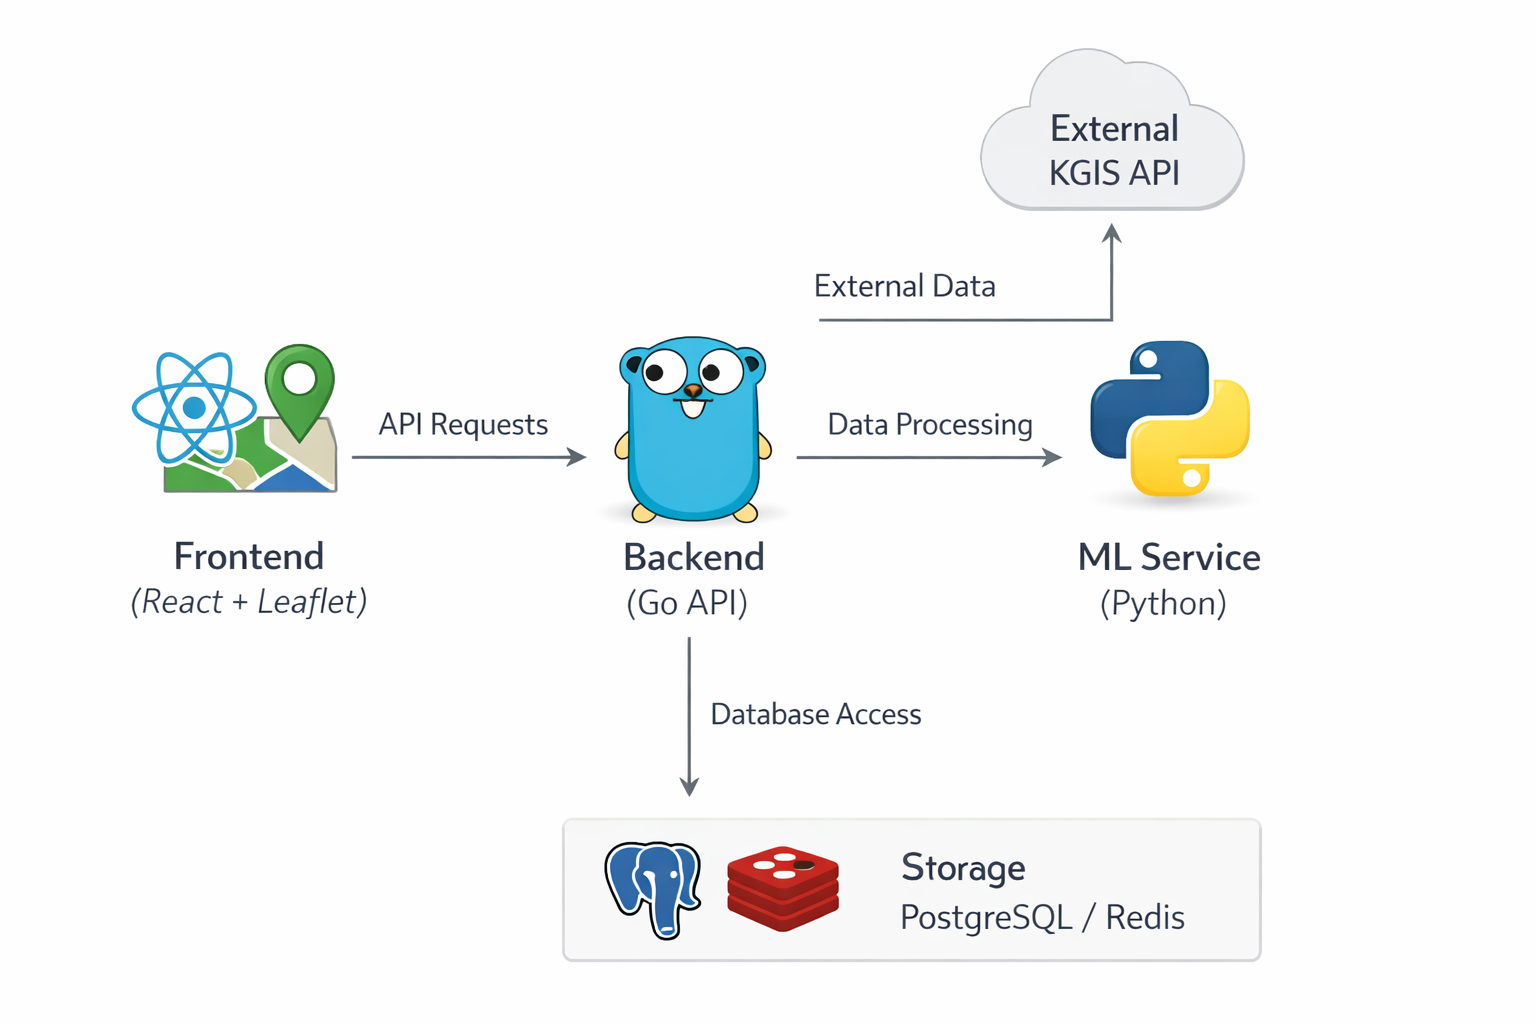
\includegraphics[width=0.45\textwidth]{architecture_landrisk.png}
}{
\fbox{\parbox[c][0.11\textheight][c]{0.42\textwidth}{\centering Add image: architecture\_landrisk.png\\System Architecture placeholder.}}
}
\caption{System Architecture}
\label{fig:architecture}
\end{figure}

\subsection{Microservices and Event-Driven Justification}
The system uses service separation by concern: backend orchestration, ML inference/satellite extraction, and frontend interaction are independently deployable. This allows isolated scaling and clearer fault domains. Caching and trace persistence decouple repeated user reads from expensive upstream geospatial operations. Although user requests are synchronous, internal pipeline segmentation provides event-like stage visibility through persisted traces and latency metrics.

\section{Component Breakdown}
\subsection{Frontend}
The frontend is a React + Vite application with Leaflet-based geospatial interaction. Users can provide input manually or by clicking on the map, then run assessment and inspect risk summary, explanation, and raw trace diagnostics. The latest UI revision adds a professionalized visual hierarchy, responsive card system, status chips, and a live activity panel with step indicators and rolling execution logs.

\subsection{Services}
\textbf{backend-go} handles request validation, orchestration, KGIS fetching, preprocessing, feature construction, ML invocation, rule-based validation, report generation, and persistence. \textbf{ml-service-python} provides satellite feature extraction and prediction APIs over a trained XGBoost model. The backend combines model outputs with deterministic validation rules (for example, water-overlap safety override) to produce final risk class and confidence.

\subsection{Shared and Infrastructure Layers}
PostgreSQL stores reports, traces, and latency metrics. Redis is used for caching and response acceleration. Docker Compose provisions frontend, backend, ML service, PostgreSQL, and Redis with health checks. This deployment model enables reproducible local and staging execution with realistic dependency orchestration.

\section{Communication and Data Flow}
\subsection{Pipeline: Request to Report}
The implemented flow is:
\begin{enumerate}
\item Input capture: frontend receives coordinates or survey identifiers and posts to \texttt{/analyze}.
\item Geospatial pull: backend fetches KGIS context and records endpoint trace metadata.
\item Preprocessing: geometry and payload normalization convert raw fields into consistent structures.
\item Satellite and ML stage: backend requests satellite features and model prediction from ML service.
\item Validation and decision: rule engine evaluates cross-source agreement and applies deterministic overrides.
\item Persistence and response: report, trace payload, and metrics are stored; response is returned to frontend.
\item Visualization: frontend shows summary, activity timeline, map context, and raw trace diagnostics.
\end{enumerate}

\begin{figure}[h]
\centering
\IfFileExists{dataflow_landrisk.png}{
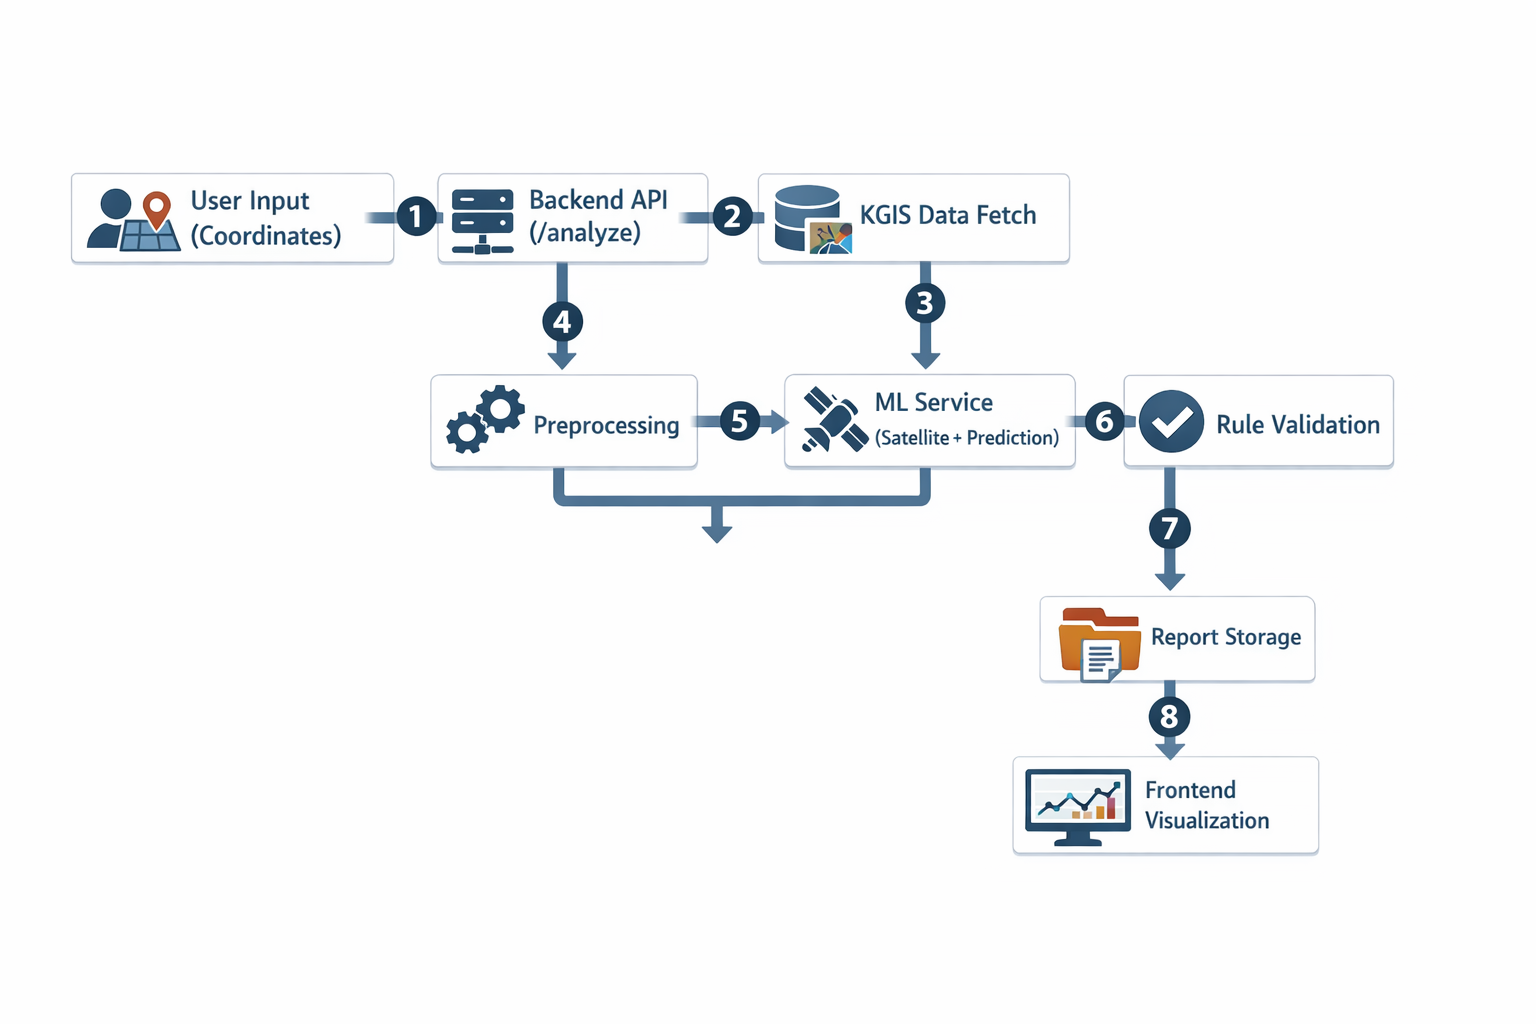
\includegraphics[width=0.45\textwidth]{dataflow_landrisk.png}
}{
\fbox{\parbox[c][0.11\textheight][c]{0.42\textwidth}{\centering Add image: dataflow\_landrisk.png\\Data Flow placeholder.}}
}
\caption{Assessment Data Flow}
\label{fig:dataflow}
\end{figure}

\subsection{Asynchrony and Reliability}
The backend enforces request-scoped timeout boundaries, uses singleflight request deduplication, and caches complete report payloads to reduce repeated expensive processing. Endpoint-level API traces and stage-level latency maps provide runtime transparency and failure diagnosis support. This combination improves reliability while preserving predictable response behavior.

\section{Technologies Used}
\subsection{Language and Runtime Choices}
Go is used for backend orchestration due to efficient concurrency, low-overhead deployment, and strong static typing for service contracts. Python is used for ML and satellite processing because scientific and model tooling are mature and easier to iterate.

\subsection{Messaging, Data, and Storage Stack}
PostgreSQL stores reports, traces, and numeric latency metrics for historical analysis. Redis serves cache entries to reduce duplicate compute and improve response times for repeated request fingerprints. The frontend is served via Nginx and built with Vite for lean client delivery.

\subsection{Scoring and Validation Logic}
The decision process combines model output and deterministic validation:
\begin{equation}
\hat{c} = \arg\max_{k} p(y=k\mid x), \quad
Risk =
\begin{cases}
\text{High}, & \text{if } WaterOverlapRatio > 0.6 \\
\text{MapClass}(\hat{c}), & \text{otherwise}
\end{cases}
\end{equation}
where confidence is adjusted using cross-source agreement between geospatial and satellite evidence.

\section{Deployment Architecture}
Deployment is container-centric through Docker Compose. Service definitions include build configuration, environment injection, health checks, dependency ordering, and networked runtime. The same command sequence builds images, starts containers, applies migrations, and seeds baseline data. This enables repeatable execution and validation across contributors.

\section{Design Decisions and Trade-offs}
\subsection{Microservices vs. Monolith}
Microservices increase operational complexity but provide cleaner scaling boundaries and isolation across UI, orchestration, and ML workloads.

\subsection{Synchronous UX vs. Background Transparency}
The user-facing API remains synchronous for simplicity, while the frontend now exposes stage-based progress and execution logs to reduce perceived opacity during longer runs.

\subsection{Strict Rules vs. Model Flexibility}
Rule-based overrides reduce model-only false confidence in sensitive scenarios (for example, strong water overlap), but can be conservative in edge cases.

\subsection{Latency vs. Traceability}
Persisting trace and metrics adds overhead, but substantially improves auditability and debugging quality. Caching and deduplication offset part of this cost.

\section{Results and Observations}
The system demonstrates stable end-to-end behavior under repeated runs, with observable per-stage latency and API trace outputs. Frontend usability improved significantly through stronger hierarchy, consistent spacing, and always-visible processing feedback. Users can now track execution state while analysis is running, reducing uncertainty and retry noise.

\begin{figure}[h]
\centering
\IfFileExists{activity_panel.png}{
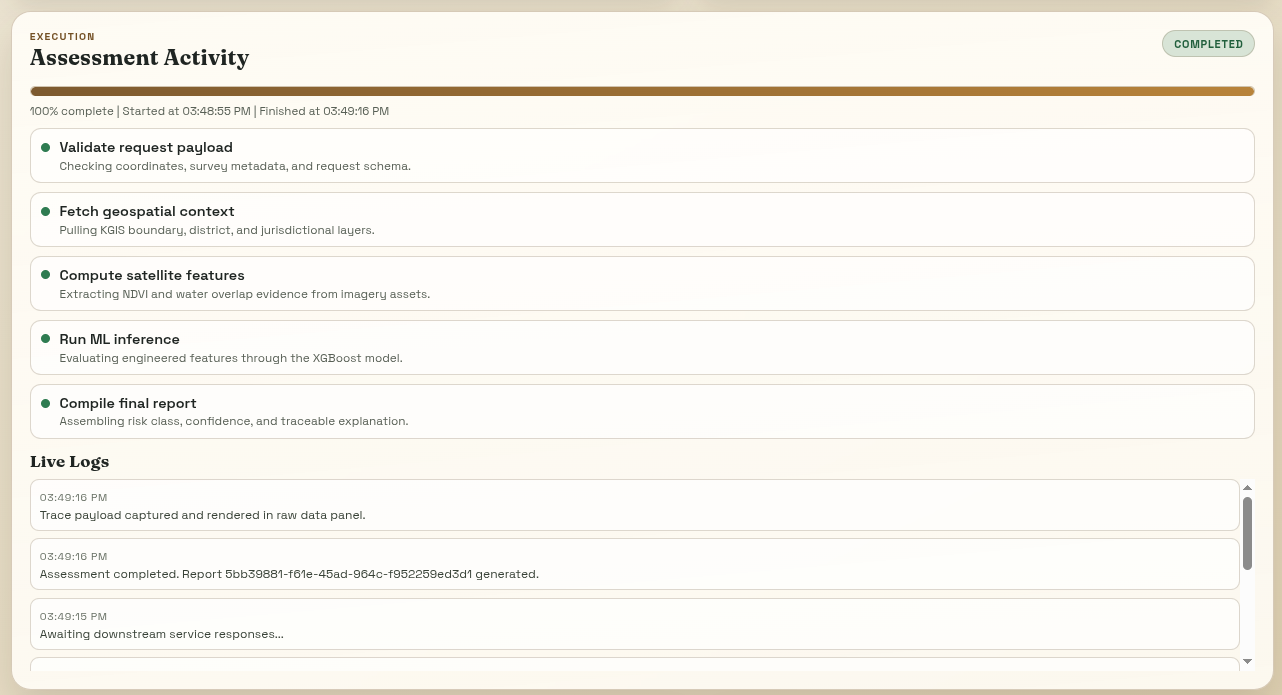
\includegraphics[width=0.45\textwidth]{activity_panel.png}
}{
\fbox{\parbox[c][0.11\textheight][c]{0.42\textwidth}{\centering Add image: activity\_panel.png\\Live activity panel placeholder.}}
}
\caption{Live Assessment Activity Panel}
\label{fig:activity_panel}
\end{figure}

\section{Evaluation Criteria Alignment}
\subsection{Criterion 1: Data Pulling and Preprocessing}
KGIS data pull, geometry normalization, and feature extraction are implemented as explicit stages with sanitization and evidence construction. Trace payloads capture source-level diagnostic details.

\subsection{Criterion 2: Technique, Logic, Data Handling, and Response Time}
The architecture uses timeout control, caching, deduplication, and latency instrumentation to balance correctness and performance. Frontend activity visualization improves operational transparency.

\subsection{Criterion 3: Accuracy and Result Validation}
Risk output is generated via model prediction plus deterministic rule checks and confidence logic based on cross-source agreement. Validation summaries are persisted for audit.

\subsection{Criterion 4: Report Quality}
The system supports structured report export (JSON/PDF), trace-backed evidence inspection, and criterion-oriented technical documentation for reproducible evaluation.

\subsection{Criterion 5: Frontend Design and Experience}
Recent UI updates improve hierarchy, consistency, responsiveness, loading states, map interaction clarity, and user trust during long-running workflows.

\section{Conclusion}
Land Risk Intelligence provides a practical reference architecture for geospatial risk assessment where explainability, runtime visibility, and usability are first-class concerns. The combined design of resilient backend orchestration, ML-powered scoring, deterministic validation, and polished frontend interaction yields a robust end-to-end assessment platform. Future work should include server-driven live stage streaming, richer accessibility instrumentation, and broader offline benchmarking for calibration and threshold tuning.

\end{document}
